\documentclass{article}
\usepackage{polski}
\usepackage{float}
\usepackage{adjustbox}
\usepackage{xcolor}
\usepackage{amssymb}
\usepackage[shortlabels]{enumitem}
\usepackage{graphicx}
\usepackage{amsmath}
\usepackage{algorithm}
\makeatletter
\renewcommand{\ALG@name}{Algorytm}
\makeatother
\usepackage{algorithmic}
\graphicspath{ {./img/} }

\title{Sprawozdanie 3 - Obliczenia Naukowe}
\author{Michał Kallas}
\date{4 grudnia 2024}

\begin{document}

\maketitle

\section{Zadanie 1}
\subsection{Opis problemu}
Napisać funkcję rozwiązującą równanie \( f(x) = 0 \) metodą bisekcji.

\subsection{Opis metody}
Metoda bisekcji jest jedną z najprostszych metod numerycznych służących do znajdowania pierwiastków funkcji. Jej podstawowe założenie opiera się na twierdzeniu Darbaux: jeśli funkcja $f(x)$ jest ciągła na przedziale $[a, b]$ i spełnia warunek $f(a) \cdot f(b) < 0$, to w tym przedziale istnieje co najmniej jeden pierwiastek. Metoda polega na iteracyjnym dzieleniu przedziału na połowę i wybieraniu podprzedziału, w którym funkcja zmienia znak. 

\subsection{Pseudokod}
\textbf{Dane:}
\begin{itemize}
  \item \( f \) – funkcja \( f(x) \) zadana jako anonimowa funkcja (ang. anonymous function),
  \item \( a, b \) – końce przedziału początkowego,
  \item \( \delta, \epsilon \) – dokładności obliczeń.
\end{itemize}

\noindent \textbf{Wyniki:}
\begin{itemize}
  \item \( r \) – przybliżenie pierwiastka równania \( f(x) = 0 \),
  \item \( v \) – wartość \( f(r) \),
  \item \( it \) – liczba wykonanych iteracji,
  \item \( err \) – sygnalizacja błędu:
  \begin{itemize}
    \item 0 - brak błędu,
    \item 1 - funkcja nie zmienia znaku w przedziale \([a, b]\).
  \end{itemize}
\end{itemize}

\begin{algorithm}[H]
\caption{Metoda bisekcji}
\begin{algorithmic}[1]
\STATE $f_a \gets f(a)$, $f_b \gets f(b)$
\STATE $e \gets b - a$
\STATE $it \gets 0$
\IF{$\text{sign}(f_a) = \text{sign}(f_b)$}
    \RETURN $(\text{Nothing}, \text{Nothing}, \text{Nothing}, 1)$
\ENDIF
\WHILE{\TRUE}
    \STATE $it \gets it + 1$
    \STATE $e \gets e / 2$
    \STATE $r \gets a + e$
    \STATE $v \gets f(r)$
    \IF{$|e| < \delta$ \OR $|v| < \epsilon$}
        \RETURN $(r, v, it, 0)$
    \ENDIF
    \IF{$\text{sign}(v) \neq \text{sign}(f_a)$}
        \STATE $b \gets r$, $f_b \gets v$
    \ELSE
        \STATE $a \gets r$, $f_a \gets v$
    \ENDIF
\ENDWHILE
\end{algorithmic}
\end{algorithm}

\section{Zadanie 2}
\subsection{Opis problemu}
Napisać funkcję rozwiązującą równanie \( f(x) = 0 \) metodą Newtona.

\subsection{Opis metody}
Metoda Newtona, znana również jako metoda stycznych, jest iteracyjną techniką przybliżania pierwiastków funkcji. Opiera się na założeniu, że funkcja może być dobrze przybliżona przez styczną do wykresu funkcji w pobliżu punktu, który chcemy znaleźć.

W każdej iteracji zaczynamy od aktualnego przybliżenia \( x_n \), obliczamy styczną do wykresu funkcji \( f(x) \) w tym punkcie, a następnie wyznaczamy punkt przecięcia tej stycznej z osią OX. Nowe przybliżenie pierwiastka, \( x_{n+1} \), to właśnie to miejsce przecięcia.
Iteracyjny wzór ma postać:
\[
x_{n+1} = x_n - \frac{f(x_n)}{f'(x_n)}
\]

Metoda Newtona jest bardzo szybka, gdy punkt początkowy jest bliski rzeczywistego pierwiastka, ale może nie działać poprawnie, jeśli początkowe przybliżenie jest dalekie lub jeśli pochodna funkcji w danym punkcie jest bliska zeru.

\subsection{Pseudokod}
\textbf{Dane:}
\begin{itemize}
  \item \( f, pf \) – funkcje \( f(x) \) oraz pochodną \( f'(x) \) zadane jako anonimowe funkcje,
  \item \( x_0 \) – przybliżenie początkowe,
  \item \( \delta, \epsilon \) – dokładności obliczeń,
  \item \( maxit \) – maksymalna dopuszczalna liczba iteracji.
\end{itemize}

\noindent \textbf{Wyniki:}
\begin{itemize}
  \item \( r \) – przybliżenie pierwiastka równania \( f(x) = 0 \),
  \item \( v \) – wartość \( f(r) \),
  \item \( it \) – liczba wykonanych iteracji,
  \item \( err \) – sygnalizacja błędu:
  \begin{itemize}
    \item 0 - metoda zbieżna,
    \item 1 - nie osiągnięto wymaganej dokładności w \( maxit \) iteracjach,
    \item 2 - pochodna bliska zeru.
  \end{itemize}
\end{itemize}

\begin{algorithm}[H]
\caption{Metoda Newtona}
\begin{algorithmic}[1]

\STATE $v \gets f(x_0)$
\IF{$|v| < \epsilon$}
    \RETURN $(x_0, v, 0, 0)$
\ENDIF

\FOR{$it = 1$ \TO $maxit$}
    \STATE $dfx \gets f'(x_0)$
    \IF{$|dfx| < \epsilon$}
        \RETURN $(x_0, v, it, 2)$
    \ENDIF

    \STATE $x_1 \gets x_0 - \frac{v}{dfx}$
    \STATE $v \gets f(x_1)$

    \IF{$|x_1 - x_0| < \delta$ \OR $|v| < \epsilon$}
        \RETURN $(x_1, v, it, 0)$
    \ENDIF

    \STATE $x_0 \gets x_1$
\ENDFOR

\RETURN $(x_0, v, maxit, 1)$
\end{algorithmic}
\end{algorithm}


\section{Zadanie 3}
\subsection{Opis problemu}
Napisać funkcję rozwiązującą równanie \( f(x) = 0 \) metodą siecznych.

\subsection{Opis metody}
Metoda siecznych jest modyfikacją metody Newtona, która nie wymaga obliczania pochodnej. Zamiast tego, przybliża jej wartość na podstawie 2 ostatnich przybliżeń.
Geometrycznie, aproksymujemy pierwiastek funkcji za pomocą stycznej do wykresu. Iteracyjny wzór ma postać:
\[
x_{n+1} = x_n - f(x_n) \cdot \frac{x_n - x_{n-1}}{f(x_n) - f(x_{n-1})}.
\]
Metoda ta wymaga dwóch początkowych przybliżeń \( x_0 \) i \( x_1 \) i jest szczególnie użyteczna, gdy obliczenie pochodnej \( f'(x) \) jest trudne lub niemożliwe.

\subsection{Pseudokod}
\textbf{Dane:}
\begin{itemize}
  \item \( f \) – funkcja \( f(x) \) zadana jako anonimowa funkcja,
  \item \( x_0, x_1 \) – przybliżenia początkowe,
  \item \( \delta, \epsilon \) – dokładności obliczeń,
  \item \( maxit \) – maksymalna dopuszczalna liczba iteracji.
\end{itemize}

\noindent \textbf{Wyniki:}
\begin{itemize}
  \item \( r \) – przybliżenie pierwiastka równania \( f(x) = 0 \),
  \item \( v \) – wartość \( f(r) \),
  \item \( it \) – liczba wykonanych iteracji,
  \item \( err \) – sygnalizacja błędu:
  \begin{itemize}
    \item 0 - metoda zbieżna,
    \item 1 - nie osiągnięto wymaganej dokładności w \( maxit \) iteracjach.
  \end{itemize}
\end{itemize}

\begin{algorithm}[H]
\caption{Metoda siecznych}
\begin{algorithmic}[1]

\STATE $fx_0 \gets f(x_0)$
\STATE $fx_1 \gets f(x_1)$

\FOR{$it = 1$ \TO $maxit$}
    \IF{$|fx_0| > |fx_1|$}
        \STATE $x_0, x_1 \gets x_1, x_0$
        \STATE $fx_0, fx_1 \gets fx_1, fx_0$
    \ENDIF
    
    \STATE $s \gets \frac{x_1 - x_0}{fx_1 - fx_0}$
    \STATE $x_1 \gets x_0$
    \STATE $fx_1 \gets fx_0$
    \STATE $x_0 \gets x_0 - fx_0 \cdot s$
    \STATE $fx_0 \gets f(x_0)$
    
    \IF{$|x_1 - x_0| < \delta$ \OR $|fx_0| < \epsilon$}
        \RETURN $(x_0, fx_0, it, 0)$
    \ENDIF
\ENDFOR

\RETURN $(x_0, fx_0, maxit, 1)$
\end{algorithmic}
\end{algorithm}

\section{Zadanie 4}
\subsection{Opis problemu}
W celu wyznaczenia pierwiastka równania \( \sin x - \left( \frac{1}{2} x \right)^2 = 0 \) zastosować wcześniej zaprogramowane metody:
\begin{enumerate}
  \item bisekcji z przedziałem początkowym \([1.5, 2]\) i \( \delta = \frac{1}{2} 10^{-5} \), \( \epsilon = \frac{1}{2} 10^{-5} \),
  \item Newtona z przybliżeniem początkowym \( x_0 = 1.5 \) i \( \delta = \frac{1}{2} 10^{-5} \), \( \epsilon = \frac{1}{2} 10^{-5} \),
  \item siecznych z przybliżeniami początkowym \( x_0 = 1 \), \( x_1 = 2 \) i \( \delta = \frac{1}{2} 10^{-5} \), \( \epsilon = \frac{1}{2} 10^{-5} \).
\end{enumerate}

\subsection{Wyniki}
\begin{table}[H]
\begin{adjustbox}{center}
\begin{tabular}{|c|c|c|c|c|c|}
    \hline
    Metoda & Parametry & Pierwiastek $r$ & Wartość funkcji dla $r$ & Liczba iteracji & Błąd\\
    \hline
    bisekcji & $a = 1.5$, $b = 2$ & 1.9337539672851562 & -2.7027680138402843e-7 & 16 & 0\\
    \hline
    Newtona & $x_0 = 1.5$ & 1.933753779789742 & -2.2423316314856834e-8 & 4 & 0\\
    \hline
    siecznych & $x_0 = 1$, $x_1 = 2$ & 1.933753644474301 & 1.564525129449379e-7 & 4 & 0\\
    \hline
\end{tabular}
\end{adjustbox}
\caption{Wyniki aproksymacji pierwiastka funkcji $f(x) = \sin x - \left( \frac{1}{2} x \right)^2$ z $\delta = \epsilon = \frac{1}{2} 10^{-5}$.}
\end{table}

\subsection{Obserwacje i wnioski}
Każda z metod dobrze poradziła sobie z przybliżeniem pierwiastka funkcji. Żadna z nich nie zwróciła błędu. 
Metody Newtona i siecznych potrzebowały tylko 4 iteracji, podczas gdy metoda bisekcji potrzebowała ich aż 16.
To wynika ze współczynników zbieżności tych funkcji - dla metody bisekcji wynosi on 1(zbieżność liniowa),
dla metody Netwona 2(zbieżność kwadratowa), a dla metody siecznych około 1.618.

Zatem, w tym przypadku metody Netwona i siecznych poradziły sobie lepiej.
Należy jednak pamiętać, że ogólnie, mimo bycia wolniejszym, metoda bisekcji jest bardziej niezawodna.
Wynika to z tego, że jest zbieżna globalnie, a nie lokalnie, jak 2 pozostałe metody.

\section{Zadanie 5}
\subsection{Opis problemu}
Metodą bisekcji znaleźć wartości zmiennej \( x \), dla której przecinają się wykresy funkcji \( y = 3x \) i \( y = e^x \). Wymagana dokładność obliczeń: \( \delta = 10^{-4} \), \( \epsilon = 10^{-4} \).

\subsection{Rozwiązanie}
Metoda bisekcji jest stosowana do znajdowania miejsc zerowych funkcji, także musimy trochę przekształcić problem.
Wiemy, że szukamy miejsca gdzie $3x = e^x$, czyli $e^x -3x = 0$. W takim wypadku wystarczy znaleźć miejsca zerowe funkcji:
$$f(x) = e^x - 3x$$

Musimy jeszcze dobrać przedziały, w których wartości funkcji mają różny znak. W tym celu posłużyłem się następującym wykresem:
\begin{figure}[H]
\centering
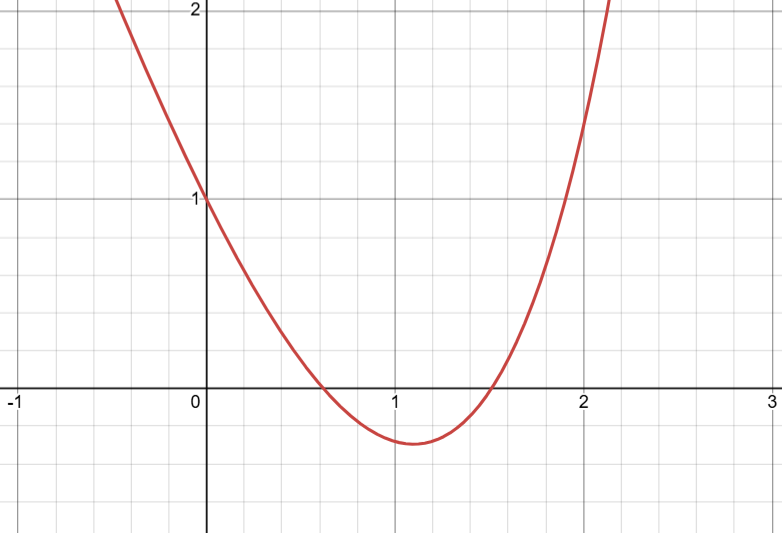
\includegraphics[width=\textwidth]{plot5.png}
\caption{Wykres $f(x) = e^x - 3x$ z Desmos.}
\end{figure}

Na podstawie wykresu można ocenić, że do znalezienia miejsc zerowych dobrze sprawdzą się na przykład przedziały $[0, 1]$ oraz $[1, 2]$.

\subsection{Wyniki}
\begin{table}[H]
\begin{adjustbox}{center}
\begin{tabular}{|c|c|c|c|c|c|}
    \hline
    Przedział & Pierwiastek $r$ & Wartość funkcji dla $r$ & Liczba iteracji & Błąd\\
    \hline
    $[0, 1]$ & 0.619140625 & -9.066320343276146e-5 & 9 & 0\\
    \hline
    $[1, 2]$ & 1.5120849609375 & -7.618578602741621e-5 & 13 & 0\\
    \hline
\end{tabular}
\end{adjustbox}
\caption{Wyniki aproksymacji pierwiastka funkcji $f(x) = e^x - 3x$ metodą bisekcji z $\delta = \epsilon = 10^{-4}$.}
\end{table}

\subsection{Obserwacje i wnioski}
Jak widać, metodę bisekcji można za sprawą prostego przekształcenia zastosować do znalezienia miejsca przecięcia się 2 funkcji.
Dzięki znajomości wykresu funkcji, zastosowanie tej metody było w tym przypadku proste i skuteczne.
Jednak, jak łatwo zauważyć, bez wiedzy o przebiegu funkcji byłoby to zadanie znacznie trudniejsze.
Nie wiedzielibyśmy gdzie szukać miejsc zerowych, a w przypadku niektórych funkcji nawet ile ich się spodziewać.

\section{Zadanie 6}
\subsection{Opis problemu}
Znaleźć miejsce zerowe funkcji \( f_1(x) = e^{1-x} - 1 \) oraz \( f_2(x) = x e^{-x} \) za pomocą metod bisekcji, Newtona i siecznych. Wymagana dokładność obliczeń: \( \delta = 10^{-5} \), \( \epsilon = 10^{-5} \).
Dobrać odpowiednio przedział i przybliżenia początkowe.

Sprawdzić co stanie się, gdy w metodzie Newtona dla \( f_1 \) wybierzemy \( x_0 \in (1, \infty] \) a dla \( f_2 \) wybierzemy \( x_0 > 1 \), czy mogę wybrać \( x_0 = 1 \) dla \( f_2 \)?

\subsection{Funkcje}
\begin{figure}[H]
\centering
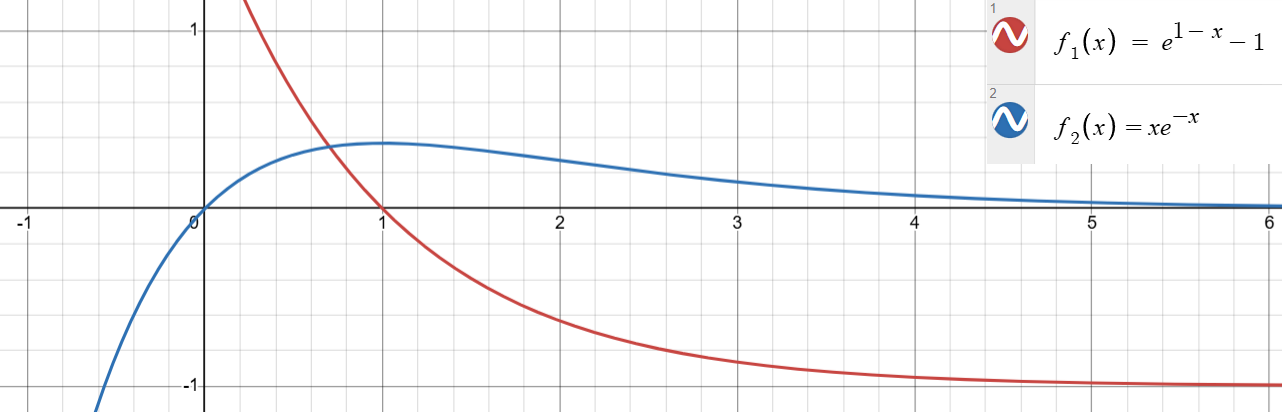
\includegraphics[width=\textwidth]{plot6.png}
\caption{Wykres \( f_1(x) = e^{1-x} - 1 \) oraz \( f_2(x) = x e^{-x} \) z Desmos.}
\end{figure}

Na podstawie wykresu możemy ocenić, że zarówno $f1$, jak i $f2$ mają jedno miejsce zerowe. Dla $f1$ jest to 1, a dla $f2$ jest to 0.

\subsection{Wyniki}
\subsubsection{Metoda bisekcji}
\begin{table}[H]
\begin{adjustbox}{center}
\begin{tabular}{|c|c|c|c|c|c|}
    \hline
    Funkcja & Przedział & Pierwiastek $r$ & Wartość funkcji dla $r$ & Liczba iteracji & Błąd\\
    \hline
    f1 & $[0, 2]$ & 1.0 & 0.0 & 1 & 0\\
    \hline
    f1 & $[0, 2.5]$ & 1.0000038146972656 & -3.814689989667386e-6 & 17 & 0\\
    \hline
    f1 & $[-10, 15]$ & 1.0000014305114746 & -1.4305104514278355e-6 & 21 & 0\\
    \hline
    f1 & $[-500, 500]$ & 1.0000020265579224 & -2.026555868894775e-6 & 26 & 0\\
    \hline
    f1 & $[-10000, 10000]$ & 0.9999983012676239 & 1.6987338189444756e-6 & 30 & 0\\
    \hline
    \hline
    f2 & $[-0.5, 0.5]$ & 0 & 0 & 1 & 0\\
    \hline
    f2 & $[-0.5, 1]$ & -7.62939453125e-6 & -7.629452739132958e-6 & 16 & 0\\
    \hline
    f2 & $[-10, 20]$ & -9.5367431640625e-6 & -9.53683411396636e-6 & 20 & 0\\
    \hline
    f2 & $[-1000, 1000.5]$ & 3.390014171600342e-7 & 3.390013022380928e-7 & 27 & 0\\
    \hline
    f2 & $[-20000, 15000]$ & 6250.0 & 0 & 2 & 0\\
    \hline
\end{tabular}
\end{adjustbox}
\caption{Wyniki aproksymacji pierwiastka funkcji \( f_1(x) = e^{1-x} - 1 \) oraz \( f_2(x) = x e^{-x} \) za pomocą metody bisekcji z $\delta = \epsilon = 10^{-5}$.}
\end{table}

\subsubsection{Metoda Newtona}
\begin{table}[H]
\begin{adjustbox}{center}
\begin{tabular}{|c|c|c|c|c|c|}
    \hline
    Funkcja & $x_0$ & Pierwiastek $r$ & Wartość funkcji dla $r$ & Liczba iteracji & Błąd\\
    \hline
    f1 & $0.5$ & 0.9999999998878352 & 1.1216494399945987e-10 & 4 & 0\\
    \hline
    f1 & $1.01$ & 0.9999999987416528 & 1.2583472042138055e-9 & 2 & 0\\
    \hline
    f1 & $1.5$ & 0.9999999984736215 & 1.5263785790864404e-9 & 4 & 0\\
    \hline
    f1 & $5$ & 0.9999996427095682 & 3.572904956339329e-7 & 54 & 0\\
    \hline
    f1 & $7$ & 0.9999999484165362 & 5.15834650549607e-8 & 401 & 0\\
    \hline
    f1 & $20$ & - & - & 1 & 2\\
    \hline
    f1 & $100$ & - & - & 1 & 2\\
    \hline
    \hline
    f2 & $0.01$ & -1.0202010000017587e-8 & -1.0202010104098596e-8 & 2 & 0\\
    \hline
    f2 & $0.8$ & -1.5586599258811135e-6 & -1.5586623553037713e-6 & 9 & 0\\
    \hline
    f2 & $20.5$ & 20.5 & 2.5628133760928222e-8 & 0 & 0\\
    \hline
    f2 & $30$ & 30.0 & 2.8072868906520526e-12 & 0 & 0\\
    \hline
    f2 & $1$ & - & - & 1 & 2\\
    \hline
\end{tabular}
\end{adjustbox}
\caption{Wyniki aproksymacji pierwiastka funkcji \( f_1(x) = e^{1-x} - 1 \) oraz \( f_2(x) = x e^{-x} \) za pomocą metody Newtona z $\delta = \epsilon = 10^{-5}$.}
\end{table}

\subsubsection{Metoda siecznych}
\begin{table}[H]
\begin{adjustbox}{center}
\begin{tabular}{|c|c|c|c|c|c|}
    \hline
    Funkcja & Parametry & Pierwiastek $r$ & Wartość funkcji dla $r$ & Liczba iteracji & Błąd\\
    \hline
    f1 & $x_0 = 0.5$, $x_1 = 1.5$ & 0.9999999624498374 & 3.755016342310569e-8 & 5 & 0\\
    \hline
    f1 & $x_0 = -2$, $x_1 = 3$ & 0.9999993443793663 & 6.556208484997939e-7 & 15 & 0\\
    \hline
    f1 & $x_0 = -5$, $x_1 = 2$ & 1.000000147648643 & -1.4764863220939617e-7 & 8 & 0\\
    \hline
    f1 & $x_0 = 0.5$, $x_1 = 1000$ & 1.0000000135075802 & -1.3507580054472612e-8 & 13 & 0\\
    \hline
    \hline
    f2 & $x_0 = -1.5$, $x_1 = 0.5$ & 1.7791419742860986e-8 & 1.779141942632637e-8 & 8 & 0\\
    \hline
    f2 & $x_0 = -1.5$, $x_1 = 4$ & 14.637124064985773 & 6.4362594367553056e-6 & 14 & 0\\
    \hline
    f2 & $x_0 = -10$, $x_1 = 1$ & 0.9999816281598148 & 0.3678794411093574 & 3 & 0\\
    \hline
    f2 & $x_0 = -10$, $x_1 = 1.2$ & 14.451486746639073 & 7.650883333713024e-6 & 12 & 0\\
    \hline
    f2 & $x_0 = -10$, $x_1 = 3$ & 2.9999911847212903 & 0.1493620828792939 & 1 & 0\\
    \hline
\end{tabular}
\end{adjustbox}
\caption{Wyniki aproksymacji pierwiastka funkcji \( f_1(x) = e^{1-x} - 1 \) oraz \( f_2(x) = x e^{-x} \) za pomocą metody siecznych z $\delta = \epsilon = 10^{-5}$.}
\end{table}

\subsection{Obserwacje i wnioski}
\subsubsection{Metoda bisekcji}
Zgodnie z oczekiwaniami metoda bisekcji znajduje pierwiastek od razu, jeśli znajduje się on na środku przedziału.
Można zauważyć, że im większe przedziały, tym większa ilość iteracji potrzebna do osiągnięcia wyniku.

Dla $f_1$ wszystkie przetestowane przeze mnie przypadki zwróciły poprawne wyniki, ale dla $f_2$ metoda bisekcji stwierdziła, że 6250 jest miejscem zerowym, podczas gdy w rzeczywistości jest to 1.
Wynika to z faktu, że wartości $f_2$ są bardzo bliskie zeru dla dużych argumentów.
Jako że są mniejsze od $\epsilon$, to metoda kończy działanie i zwraca niewłaściwy wynik.
Jest to całkiem groźne, jako że nie mamy informacji o błędzie.

\subsubsection{Metoda Newtona}
W przypadku $f_1$ dla odpowiednio małych $x_0 > 1$ metoda Newtona zwraca poprawne wyniki, ale zauważalny jest szybki wzrost ilości iteracji.
Dla większych punktów początkowych pochodna jest zbyt bliska zeru i dostajemy błąd.

Dla $f_2$, dla punktów początkowych bliskich pierwiastkowi metoda Newtona zwróciła poprawne wyniki.
W przypadku $x_0 = 1$ dostajemy błąd, jako że $f_2'(1) = 0$, co oznacza że styczna jest równoległa do osi OX.
Dla większych $x_0$ metoda też nie zadziałała, jako że wartość funkcji była zbyt bliska zeru i został zwrócony niepoprawny wynik, podobnie jak w przypadku metody bisekcji.

\subsubsection{Metoda siecznych}
Dla $f_1$ wyniki są zadowalające. Metoda siecznych zdaje się radzić sobie lepiej niż metoda Newtona.

Jednakże, dla $f_2$ pojawiło się duży niepoprawnych wyników. Należy w tym przypadku unikać $x_1 > 1$, gdyż prowadzą one do fałszywych rezultatów.
Dla ujemnych $x_0$ sieczna przecina się z osią OX bardzo blisko $x_1$, co prowadzi do końca algorytmu przez warunek z $\delta$.

\subsubsection{Podsumowanie}
Powyższe eksperymenty pokazują nam, że musimy być bardzo uważni korzystając z metod aproksymacyjnych.
Bez dobrej analizy przebiegu funkcji nie będziemy wiedzieli gdzie szukać miejsc zerowych i jakie wyniki możemy odrzucić jako niepoprawne.

Metody Newtona i siecznych wymagają bardzo starannie dobranych parametrów w celu otrzymywania sensownych wyników.
Co istotne, nawet najbezpieczniejsza, globalnie zbieżna metoda bisekcji zwracała w eksperymentach niepoprawne wyniki.
Nie możemy po prostu wybrać ogromnego przedziału i liczyć na znalezienie pierwiastka, bo takie podejście może prowadzić do błędów.
Trzeba bardzo uważać na złośliwe funkcje.

\end{document}
